\documentclass[letterpaper]{article}
\usepackage{iccc}

\usepackage{graphicx}
\usepackage{times}
\usepackage{helvet}
\usepackage{courier}
\pdfinfo{
	/Title (Anything2vec: generalizing word2vec-like embedding for movie tropes via the use of meaningful contexts)
	/Subject (Proceedings of ICCC)
	/Author (ICCC)}
% The file iccc.sty is the style file for ICCC proceedings.
%

%\title{Anything2vec: generalizing word2vec via the use of meaningful
%	contexts}
% Add something about its application to trope description - JJ 
%\author{Dan Ventura\\
%Computer Science Department\\
%Brigham Young University\\
%Provo, UT 84602  USA\\
%ventura@cs.byu.edu\\
%}
\setcounter{secnumdepth}{0}

\begin{document} 
	% \maketitle
	\begin{abstract}
		\begin{quote}
			% From the old paper:
			%   Word2vec has been a very successful algorithm that is able to give a
			% semantic representation to words on a corpus based in the context
			% they appear. In this paper we will try to extend this concept to
			% other {\em unordered} contexts. We will try to define this context
			% for movie (and TV) tropes.
			In this article, we present a generalized approach to extend the use of word2vec for non-traditional Natural Language Processing. To exemplify the idea, we use the tvtropes data set to create a text corpus in order to provide contextual information to any data. Two different approaches have been made: the first called N-Grams Permutation Model and the second Database Like Reinforcement Model. We have compared both approaches with a model based on text written by humans and we have verified that in the best case the model based on artificial corpus improves accuracy on the one created by humans by 45.2\%.
		\end{quote}
	\end{abstract}
	
	% From the old paper:
	% What are tropes and why we are interested
	
	% We need to find an embedding for tropes that allows us to do trope arithmetic and also process them, and movies in which they are used, in an uniform way.
	
	% We propose trope2vec
	
	% We analyse how it allows to explore the trope space and find
	% similarities between them.
	
	\section{Introduction}
	
	% Some help from: https://www.nature.com/scitable/topicpage/scientific-papers-13815490/
	
	% First, provide some context to orient those readers who are less familiar with your topic and to establish the importance of your work.

    %How would they use it? - JJ
   With growing diversity and quantity of entertainment content such as movies, video games, TV series or books, also growing the interest in creating higher quality entertainment content.
   Each of these content uses resources and techniques that are studied and used repeatedly and they are called tropes. Being able to characterize these tropes so that they can be used within a computer algorithm can be very interesting for those creators who perform this type of artistic work. A frequent technique to organize information to use with computer algorithms is to provide each piece of information with an associated multidimensional vector. One of the most used techniques in recent years for vector representations of words is word2vec \cite{mikolov2013}.
   With this technique, vector obtained for each word has the ability to save information of its environment. This vector is called embedding vector.  % REFERENCE!!!! - JJ
   Another interesting feature of embeddings vectors is that it is possible to perform concept arithmetic. For example, it would be possible to subtract and add vectors so that we obtain another vector resulting from the operation: Paris - France + Italy = Rome. However, to apply this algorithm, it is necessary to have a sufficiently large corpus written in natural language. Some examples of this frequently used corpus are Wikipedia or Google News dumps, usually greater than 1GB of plain text. See \cite{google-word2vec} to obtain more examples. \\
   % tHIS COMPARISON IS NOT YOURS (NOT TO MENTION IRRELEVANT). Please add a reference.
   % If this is what you want to do, layout an use case for this kind of things. - JJ
   
   But, it would be possible to apply word2vec to represent the relationships between tropes and films? With this work, we want to demonstrate that it is possible to obtain embeddings vectors using word2vec of an artificially created corpus. To demonstrate this idea we will use data from films and tropes obtained from tvtropes.org website. TV Tropes is a collaborative website created in 2004 to share information about tips, narrative or cinematographic techniques
   used in creative works such as movies, TV-series, advertising,
   videogames, sports, comics or books; the latest iterations even include
   {\em real life} tropes. Tvtropes.org defines tropes as:
   "a storytelling device or convention, a shortcut for describing
   situations the storyteller can reasonably assume the audience will
   recognize." Articles to describe tropes are written usually with a very
   expressive and non-formal vocabulary. 
   Each film, TV series or other fiction elements usually include a description and a list of associated tropes. Tropes pages usually contain a description followed by a list
   of films or a narrative resource that uses this trope.
    
	% Second, state the need for your work, as an opposition between what the scientific community currently has and what it wants.
	
	On the other hand, other works like \cite{kazama2018} have shown that it is possible to use word2vec to obtain vectors from non-NLP information sources. In our case, we want to use word2vec to obtain vectors from non-NLP sources of information through two different methods and demonstrate that these artificially created texts can provide greater precision than text written by humans. If the artificial corpus is correctly constructed, it should produce some embedding vectors with the capacity to offer us the right arithmetic of concepts. We want the word representation to have the following characteristics: 
	
	\begin{itemize}

	\item That includes the context of the trope
	\item relatively compact
	\item capable of doing arithmetic
	\item uniform for tropes and movies.
		
    \end{itemize}  
	   
	% Third, indicate what you have done in an effort to address the need (this is the task).

    In order to solve the problem, we have downloaded film data from word2vec using Tropescraper \cite{doi:10.1111/exsy.12525} to easily dump tvtropes content.
    % This is methodology. This shouldn't be in the introduction - JJ
     Then we have extracted a subset of films whose number of tropes is less than a certain threshold. From this subset of films and tropes, we have built an artificial corpus on which to apply the word2vec algorithm and generate embeddings. To evaluate that the subset of tropes is representative, we have verified that 92\% of the subset are among the most frequently used tropes. With the obtained vectors we have generated a classification to verify the correspondence between embeddings and real films-tropes relationships. From the vectors that represent the tropes, we have created a vector for the film. As a result, we have verified that the artificially generated corpus fulfills the desired objective. The obtained graphic representation shows that obtained clusters are correlated with real relationships observed between tropes and between tropes and films.\\
 
% How we want to solve that problem: we think that an adaptation of word2vec should be possible
% This is what you say above - JJ	
% How we do it:
% * Methodology for creating the context of every trope
% * Methodology for representing movies using trope vector
% * How we evaluate the goodness of the set of movies/tropes chosen.

% Our results
% * Clustering
% * Graph representation
% * Movie representation
% * Example of synthetic movie generation.
	
	
	% Finally, preview the remainder of the paper to mentally prepare readers for its structure, in the object of the document.

	The rest of the paper is organized as follows. Next we present the
	state of the art in using embedding for problems other than language
	processing, as well as an overview of the use of tropes for narrative
	generation. The methodology is presented next in Section
	\ref{sec:met}, with results presented in Section \ref{sec:res}
	followed by the conclusion that closes the paper.
	
	
	\section{State of the art}
	
	Unlike systems such as MovieLens \cite{10.1145/2827872}, which focus
	on recommendation, our ultimate
	interest in representing movie tropes lies in the possibility of
	generating narratives \cite{10.5555/931357} that are optimal from some point of view (mainly
	coherence) from a set of tropes. Out of all the possible methods to
	generate narratives \cite{van2019narrative} this is one that has
	probably been explored the least; Sullivan et
	al. \cite{10.1145/3235765.3235819} used tropes in the tarot deck to
	generate narratives via combinations, but other than that, in general
	the presence of tropes has been used more for evaluation of generated
	narratives \cite{gervas2012story} that as part of the generation
	itself; in general, tropes are understood as constraints for
	characters or plots \cite{Thompson18NarrativeEvents}, but, of course,
	there are many kind of tropes and some of them can be converted
	directly into plots; for instance, {\sf AgeStereotypicalFood} informs
	of the fact that eating or talking about food will be introduced into
	the narrative.
	
	This work has been inspired by other that have used
	word2vec-like embeddings for purposes that are totally
	unrelated to natural language; a good survey is presented in
	\cite{nonnlp19}. In general, creating embeddings out of data
	is done with several purposes: reducing dimensionality, but
	also trying to create a data representation with semantics; as
	a side effect, this data representation will enable ``content
	arithmetics''. In our previous work
	\cite{doi:10.1111/exsy.12525} we used a direct representation
	of tropes; every dimension in a vector represented a trope,
	once less frequent ones had been excluded. However, this left
	out many possibly meaningful tropes, and still the size of the
	vectors was huge, representing its own challenge when using
	them in a deep learning algorithm.
	
	This was one of the intentions of Kazama et al. in
	\cite{kazama2018}, which is actually the paper that inspired
	our work. The content they wanted to represent was the concept
	of ``regional cuisine'', so that a regional cuisine embedding
	could be added or subtracted from the embedding of a dish to
	create a new, equivalent one in that new regional
	environment. The kind of data they were working with is
	similar to the one we use in this paper: dish ingredients. As
	in our case, there's no natural order in the ingredients, but
	unlike our case, the amount of ingredients that are used in a
	dish are really limited, at least if you exclude
	seasoning. But they achieved their objective: being able to do
	recipe arithmetics, but also create meaningful maps of food
	that can be used in deep learning or any other environment.
	
	Most other applications are similar, in a way, to this one,
	and most of them are also recent. There was a publication in
	the Twitter engineering blog \cite{twitter:embeddings},
	apparently pointing to their use studying the social networks
	of users. Initial work was done by Grbovic et al. applied it to product recommendation
	\cite{Grbovic2015}, Vasile et al. applied it to product
	recommendation systems \cite{vasile2016} while McAuley et
	al. \cite{DBLP:journals/corr/McAuleyPL15} used embedding
	arithmetics to find complementary products to others that had
	been already purchased; these articles were
	probably ones of the first to use this kind of
	representation.
	
	Word embeddings to create clustering, however, go back at
	least to Kohonen's work in the 90s
	\cite{kohonen1997exploration}, which tried to create
	embeddings by assigning a word a vector created from averaging
	randomly created vectors initially assigned to its neighboring
	vectors. This work was extended to ant clustering algorithms
	to create word clusterings by Ramos et
	al. \cite{DBLP:journals/corr/abs-cs-0412075}.
	
	The fact that the variety of data embeddings have been applied
	to, as well as the kind of applications created with is so
	wide, has encouraged us to apply it to the study of movies via
	their tropes, as well as its eventual optimization.
	
	\section{Methodology}
	\label{sec:met}
	
	
	To demonstrate that artificially created texts based on films and tropes relationships, can provide greater precision to obtain vectors using word2vec than text written by humans, two different approaches have been analyzed:
	\begin{enumerate}
	\item The First one consists of generating the corpus through tropes permutations and adding film names in each phrase. In order to simplify the process of creating and verifying the accuracy, we have selected films with a maximum number of tropes per film. Table \ref{tab:corpusSize} shows how the maximum number of tropes affects the size of the corpus.
	
%	\item The second method consists of creating the corpus through relationships reinforcement between tropes and films as if it were a relational database. To compare both approaches, we have selected the same films for both methods.
	\end{enumerate}
	
	\subsection{Approach 1: N-Grams Permutation Model}

	This approach (NG Model) uses tropes permutation as a method of creating corpus phrases. Next to the selection of permuted tropes, the name of the film is added in order to connect the film with its tropes. In this approach, the relationship between film and their tropes is lighter, since the film's name will be next to nine other tropes. The relationship between the different tropes is also not reinforced by any criteria, we simply sort the group of tropes randomly. Before deciding which maximum number of tropes per film and the size of the phrase (n-gram) is most appropriate, we have performed different tests. Table \ref{tab:corpusSize} shows different values for MAX\_TROPE and NGRAM\_SIZE. After different tests, we have decided to take the values 15 and 9 respectively to create the corpus. We take this
	initial limit since we will generate all the variations
	without repetitions of 15 elements taken in groups of 9
	elements. This method can give us enough size corpus to train the model using word2vec algorithm. This method consists of the following steps:
	
	\begin{enumerate}
	\item Getting film data from tvtropes.org and their associated tropes using Tropescraper. % using... - JJ
	\item Select films with a number of tropes less than a certain threshold
	\item Create phrases from permutations of the tropes associated with each movie and including film name in each phrase
	\item Build word2vec model. After that, we will obtain an embedding vector for each film and trope
	\item Generate accuracy checklist  % What?  JJ
	\item Check model accuracy using generated checklist
	\item Visualize tropes vector space to detect clusters and possible data organization.
	\end{enumerate}

	% Main idea here is that the artificial corpus will represent the true as much as possible. ¿how we can achieve that?
	% We need a parameter that let us reinforce more real relationships between elements that are stronger. For example, in case of films,
	% we can use a value of film popularity to write more times in corpus information about a blockbuster film. We have to do the same with 
	% es like tropes. More relevant tropes will be them who appear more times in films, so these tropes have to appear more times in 
	% corpus. Ideal situation will be that artificial corpus emulate real conextions faithfully.\\
	% Let's use imdb blockbuster films sort by votes. Votes will be the number to reinforce more in corpus films that have more votes.	 
	% we can apply an incremental approach to do that, creating verification check lists to see if certain part of the corpus fits reality. 
	% for next paper version

    \subsubsection{Getting film data}
		
	\begin{table}[t]
		\centering
		\begin{tabular}{|p{0.24\linewidth}|p{0.18\linewidth}|p{0.18\linewidth}|p{0.18\linewidth}|}
			\hline
			\textbf{(Max\_Tropes, Ngram\_Size)}& \textbf{(16,9)} & \textbf{(15, 9)} & \textbf{(12,7)}\\
			\hline
			\hline
			Tropes Subset Size&8125&7383& 5500\\
			\hline
			Film Subset Size&2686&2380& 1674\\
			\hline
			Corpus File Size (MB)&747&264& 32\\
			\hline
			Word2vec Model file Size(MB)&5.6&4.9&4.9\\
			\hline
			Vocab Size& 7078 & 6173 & 4653\\
			\hline
			Words in train file& 48893099 &17386514&2056372\\
			\hline

		\end{tabular}
		\caption{Characteristics of different corpus sizes and word2vec models created by varying MAX\_TROPES and NGRAM\_SIZE (word2vec argument min-count = 5, MIN\_TROPES = 2)}
		\label{tab:corpusSize}
	\end{table}
	
After downloading films and tropes data from tvtropes.org (on date 13th December 2019) and processing the obtained information, we get 12360 movies and 26742 (25405 after removing repeated) tropes. The film with a higher number of tropes has 1028 tropes and the film with the minimum number of tropes has 0 tropes.

\subsubsection{Select films and tropes}
\label{sec:select-films}

From all these data we must filter repeated elements and get only those films that have between 15 and 2 tropes and their associated tropes. After selecting this group of films we get 2380 films and 7383 tropes.
Figure \ref{fig:tropesdistributionasociatedtofilms} shows the distribution of films by the number of tropes and the cumulative total of tropes. Here we can see how for a value of 250 in the maximum number of tropes in a film 98.4\% of the tropes are covered. In order to check if our subset of tropes is relevant, we sort the tropes by frequency of occurrence. We verify that in our subset is 99.2\% of the most popular tropes, so we can consider it a representative subset. In order to obtain the most popular tropes, we obtain all film-trope pairs, a total of 599341 different pairs. Counting the number of times that each trope appears in the film-trope pairs list, we will obtain the use frequency of each trope.

    \begin{figure}
\centering
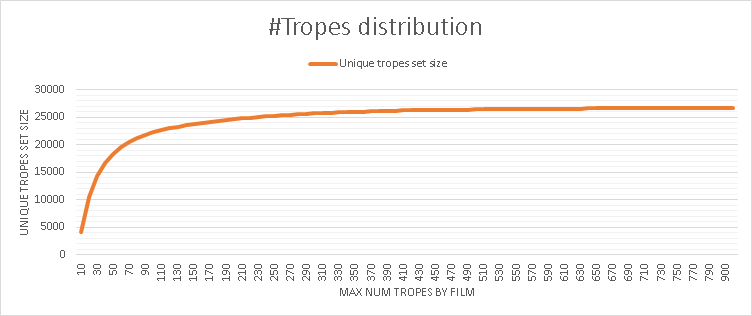
\includegraphics[width=1\linewidth]{../images/tropes_distribution_chart.png}
\caption{Accumulative distribution of tropes associated to films}
\label{fig:tropesdistributionasociatedtofilms}
\end{figure}

\subsubsection{Create corpus by tropes permutation}
The next step consist of creating an artificial corpus through the permutation of sets of M values taken from N in N. M corresponds to the film number of tropes  (MAX\_TROPES) and N with the size of the phrase or NGRAM-SIZE. table \ref{tab:corpusSize} shows different sizes of NGRAM\_SIZE and MAX\_TROPES. We decided to use the values of 15 and 9 respectively since it offers us a corpus size that we consider may be suitable for training. Within each sentence, we include the name of the film by way of creating the relationship between both, films and their tropes. 
For movies with less than 9 tropes, we simply include all of them along with the name of the movie. Finally, each sentence is randomly sorted.

\subsubsection{Build word2vec model}

The word2vec algorithm is applied to the generated corpus. For this, we use the package \cite{git-hub-word2vec} developed by the creators of the article \cite{mikolov2013}. In the model creation process, we use the bag-of-words algorithm, a 200 dimensions vector of size, a window of size 5 and a min-count of 1 (words that are repeated less than once are eliminated) as main parameters. The table \ref{tab:variations-with-min-count-argument-15-9} shows how the MIN COUNT parameter affects the Vocab Size. In our case, since the corpus is created artificially, we do not want to eliminate the less frequent words and we have used to stop the creation of all models with the MIN COUNT value = 1.
	
	% There's no need to say what to do; focus on the results and the
	% methodology. Mechanical steps can be explained in the repository.
	

\subsubsection{Visualize tropes vector space}
In order to visualize the tropes vector space, we have analyzed the different generated clusters using a modified version of the demo-classes.sh script from \cite{git-hub-word2vec}. 
We have independently visualized some of these groups in a two-dimensional space using the cluster-visualization.py script that makes use of the gensim, matplotlib libraries and the Principal Component Analysis algorithm from sklearn python library. We have also verified by taking some clusters that the elements included in a grouping are strongly connected on the tvtropes.org website.

% a big TBD -----------------------------------------------------------------------------

\section{Results}
	\label{sec:res}
	
	% Accuracy
	

        % Clusters

        % This might make sense, but I'm not totally sure...
        
    Another way to verify the quality of the embedding vectors is to check the quality of the clusters obtained. This method introduces the complexity of needing an expert who knows the nature of the data to perform the verifications of the clusters. We show the results obtained using the k-means algorithm of \cite{git-hub-word2vec} package for 1024 classes.   In our case, we have analyzed several of the clusters obtained and these are the results. First, we have visualized the vectors in a 2-dimensional space. Figures \ref{fig:cluster-db-323-visualization-zoom-out} and \ref{fig:cluster-ng-827-visualization-zoom-out} show an overview of the space while showing the location of the labels corresponding to cluster Model DB 323 and Model NG 827 respectively. Figures \ref{fig:cluster-db-323-visualization-zoom-in}, and \ref{fig:cluster-ng-827-visualization-zoom-in}. show a detail of some of the labels of cluster 323 of Model DB and cluster 827 of model NG. Table \ref{tab:cluster-example} shows the elements of two selected clusters: cluster number 323 for Model DB and cluster number 827 for Model NG. After analyzing the elements of the selected clusters we have verified that the elements of the DB 323 cluster have in common their most frequent trope "Blatant Lies". Of the 7 elements belonging to cluster \#323 of the DB Model, 5 of them are movies ("The Devil and Miss Jones", "Everybodys Fine", "Seven Years In Tibet", "Black jackets" and "Abducted in plain sight") and two others are tropes ("Blatant Lies" and "Villainous Breakdown"). The two movies in cluster have "Blatant Lies" as one of their main tropes, however, the trope "Villainous Breakdown" does not appear in any of them. From this first cluster, we can extract that all the elements are strongly interconnected except the "Villainous Breakdown" trope with which we have not found the relationship. In the case of cluster 827 of the NG Model, we have observed that: The "Ghosts Of Mississippi" movie only contains the "Cameo" and "Historical hero upgrade" tropes and film "Seven Years in Tibet", continent tropes "Dueling Movies", "Historical Hero Upgrade", "Scaling the summit" and "Training the peaceful villagers". For this second cluster, we can see that the elements are bound with less force. This makes sense since the way of building the corpus is very different. In the DB Model, relations between entities are strongly reinforced by putting emphasis on the top trope. However, the NG model relationships are somewhat lighter and thus is reflected in the resulting clusters.


\section{Conclusions, discussion and future work}


\bibliographystyle{iccc}
\bibliography{iccc}

\end{document}
